\chapter{Basic derivatives and antiderivatives}
\label{sec:basic_derivatives_and_integrals}

This chapter covers the derivatives and integrals of common functions: polynomials, exponential, and logarithms; focusing on their geometrical interpretation.

\prerequisites{binomial theorem (\cref{appendix:binomialexpansion}), basic trigonometry, derivatives, and integrals}

\paragraph{Terminologies:} The integral refers to the area under the curve. The antiderivative refers to the function $A(x')$ that outputs the area under the curve from $0$ to $x'$.

\section{Basic rules}
\label{sec:trivial_rules}

\index{derivatives!chain rule}
\paragraph{The chain rule} The Leibniz' notation treats derivative as fractions; thus, we can cancel terms (\cref{eq:prechainrule}). We exploit this property to find derivatives of composite functions. Consider two functions $f(x)$ and $g(x)$, the derivative of $f(g(x))$ can be found by a simple substitution. First let $g(x) = u$.
\begin{equation*}
	\odv*{f(g(x))}{x} = \odv{f(u)}{x}.
\end{equation*}
Let $1 = \odv{u}{u}$, then
\begin{equation*}
	\odv*{f(u)}{x} = \odv*{f(u)}{x} \times 1 = \odv{f(u)}{x} \odv{u}{u}.
\end{equation*}
Perform a change of denominator, then substitute back $u = g(x)$:
\begin{equation*}
	\odv*{f(g(x))}{x} = \odv{f(u)}{u} \times \odv{g(x)}{x}.
\end{equation*}
This is what we call the chain rule, or more generally
\begin{equation}
    \odv{y}{x} = \odv{y}{u} \times \odv{u}{x}. \label{eq:chainrule}
\end{equation}
where $u$ is a function of $y$.

The chain rule holds the intuition of how rate of changes relate to each other. E.g., the cheetah's speed is $10$ times the bicycle's speed, which is $4$ times the walking speed. The ratio between the cheetah's speed compared to walking speed would obviously be $10\cdot 4 = 40$:
\begin{equation}
    \odv{\textrm{Cheetah}}{\textrm{Walking}} = \odv{\textrm{Cheetah}}{\textrm{Bicycle}} \times \odv{\textrm{Bicycle}}{\textrm{Walking}}.
\end{equation}

\index{integral constant}
\paragraph{Integral constant} In \cref{sec:function_in_the_haystack}, each time we evaluate the antiderivative, we add an initial condition term, i.e., $v_0$ and $r_0$. So for any function $f(x)$,
\begin{equation}
    \int f(x)\odif{x} = A(x) + C
\end{equation}
where $C$ is any constant. However, \cref{theorem:fundamentalthmofcalc2} still holds for integrals with bounds.
\begin{center}
	\textbf{
		\large Always add an integral constant after evaluating the antiderivative
	}
\end{center}

\index{integrals!of an infinitesimal}
\paragraph{Integral of the infinitesimal} The antiderivative of the small rectangles $\odif{x}$ is just the total rectangle $x$ plus the integral constant $C$. 
\begin{equation}
    \int \odif{x} = x + C.
\end{equation}

\paragraph{Rules of equality} If two arguments are equal, their derivatives and antiderivatives w.r.t. the same variable must also be equal.
\begin{equation*}
    \textrm{If}~f = g,\textrm{ then }\odv{f}{x} = \odv{g}{x},\textrm{ and }\int f\odif{x} = \int g\odif{x} + C
\end{equation*}

\index{derivatives!of a constant}\paragraph{Derivative of a constant} A constant doesn't change; thus, the derivative of a constant is zero. 
\begin{equation}
    \odv*{(c)}{x} = 0.
\end{equation}

\section{Linearity of differentiation and integration}
\label{sec:diff_int_linearity}

\begin{figure}[ht]
    \centering
    \begin{subfigure}[t]{0.75\textwidth}
        \centering
        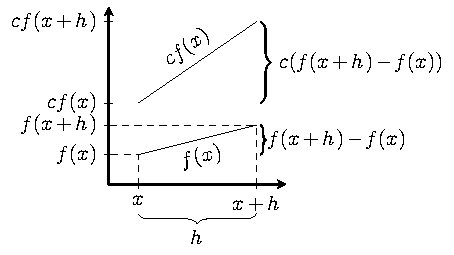
\includegraphics{basicderivativesandintegrals/derivativeconstantmultiple}
        \caption{for derivatives}
        \label{fig:derivativesconstantmultiple}
    \end{subfigure}
    \begin{subfigure}[b]{0.36\textwidth}
        \centering
        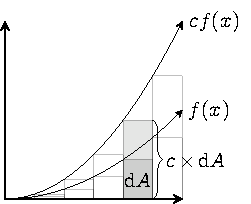
\includegraphics{basicderivativesandintegrals/integralconstantmultiple}
        \caption{for integrals}
        \label{fig:integralsconstantmultiple}
    \end{subfigure}
    \caption{Constant multiple rules}
\end{figure}

A \textbf{linear} mathematical entity are defined as anything that is compatible with addition and scaling. E.g., for a function $f(x)$ to be linear, it must obey
\begin{enumerate}[noitemsep]
    \item Additivity: $f(x + y) = f(x) + f(y)$
    \item Homogeneity of degree one: $f(ax) = af(x)$ for all constant $a$
\end{enumerate}
The simplest linear function there is, is a line that passes through the origin: $f(x) = ax$, in which
\begin{gather}
    f(x + y) = a(x + y) = ax + ay = f(x) + f(y), \\
    f(cx) = a(cx) = c(ax) = cf(x).
\end{gather}
Because this property, we associate a line with being linear. However, linearity doesn't have to always refer to lines.

Both derivatives and integrals are linear; for any function $f(x)$, $g(x)$, and constants $a$, $b$, the following rules follow.
\index{derivatives!constant multiple rule}\index{integrals!constant multiple rule}\paragraph{The constant multiple rule:}
\begin{align}
    \odv*{(af(x))}{x} &= a\odv{f(x)}{x}, &\alc[0.3]{Illustrated in \cref{fig:derivativesconstantmultiple}}\label{eq:derivativesconstantmultiple} \\
    \int af(x)\odif{x} &= a\int f(x)\odif{x}. &\alc[0.3]{Illustrated in \cref{fig:integralsconstantmultiple}}\label{eq:integralsconstantmultiple}
\end{align}
The geometrical interpretation of these two rules are very simple. When a function is multiplied by a constant $c$, its value is increased by a factor of $c$ everywhere. The slope must also be increased by $c$, and thus the function's area also.
\index{derivatives!sum rule}\index{integrals!sum rule}\paragraph{The sum rule:}
\begin{align}
    \odv*{(f(x) + g(x))}{x} &= \odv*{f(x)}{x} + \odv*{g(x)}{x}, \label{eq:derivativesumrule}\\
    \int f(x) + g(x)\odif{x} &= \int f(x)\odif{x} + \int g(x)\odif{x}. \label{eq:integralssumrule}
\end{align}
I.e., adding two functions increases its slope, thus also increasing its area under the graph.

\section{Derivatives and antiderivatives of polynomials}

Now that we've discussed the \enquote{trivial rules}, we're ready to tackle the easiest family of functions: the \textbf{polynomials}\index{polynomials}. They're in the form
\begin{equation}
    f(x) = a_0 + a_1x + a_2x^2 + a_3x^3 + \dots. \label{eq:polynomial_form}
\end{equation}
Let's focus on the antiderivative first; we'll see later how the antiderivative of polynomials can be found with just a simple substitution trick.

The form mentioned in \cref{eq:polynomial_form} is quite useless if we want to make progress. We can break it down by using the linearity of derivatives:
\begin{align}
    \odv{f(x)}{x} &= \odv*{(a_0 + a_1x^1 + a_2x^2 + a_3x^3 + \dots)}{x} \\
    &= a_1\odv{x^1}{x} + a_2\odv{x^2}{x} + a_3\odv{x^3}{x} + \dots.
\end{align}
Now we're left with derivatives of \emph{monomials} in the form of $x^n$. So let's do that instead.

\subsection{Derivatives of monomials: the power rule}
\label{sec:derivativespowerrule}

The method of increments allow us to quickly evaluate the derivative of $x^n$.
\begin{equation}
    \odv*{(x^n)}{x} = \lim_{h \appr 0}\frac{(x + h)^n - x^n}{h}.
\end{equation}
By using the binomial expansion (\cref{appendix:binomialexpansion}), 
\begin{align}
    &= \lim_{h \appr 0}\frac{\left(\sum_{k = 0}^n{n\choose k}x^{n - k}\cdot h^n\right) - x^n}{h} \\
    &= \lim_{h \appr 0}{{n\choose 0}x^nh^0 + {n\choose 1}x^{n - 1}h^1 + {n\choose 2}x^{n - 2}h^2 +\dots {n\choose n} + x^0h^n - x^n\over h} \\
    &= \lim_{h \appr 0}\frac{x^n + nx^{n - 1}h^1 + {n\choose 2}x^{n - 2}h^2 + \dots + h^n -x^n}{h} \\
    &= \lim_{h \appr 0}nx^{n - 1} + {n\choose 2}x^{n - 2}h + {n\choose 3}x^{n - 3}h^2 + h^{n - 1}
\end{align}
The terms with $h$ vanishes when $h \appr 0$; therefore,
\begin{equation}
	\odv*{(x^n)}{x} = nx^{n - 1}, \label{eq:power_rule}
\end{equation}
which is what we call the power rule. Because the binomial theorem work for all real numbers, this is true for any powers of $n$. But what about the geometrical interpretation given?

Let's now focus on the geometrical interpretation of the derivative of $x^2$: a function that represents the area of a square sidelength $x$. Its derivative then represents the ratio between the change in $x$, and the change of area when the sidelength is increased by $\odif{x}$.

\begin{figure}[b]
    \centering
    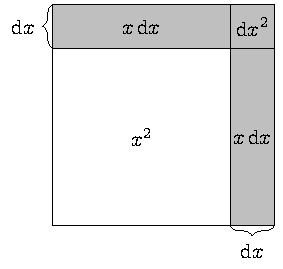
\includegraphics{basicderivativesandintegrals/xsquaredpowerrule}
	\caption{Interpretation of $\odv{x^2}{x}$ ($\odif{x}$ exaggerated)}
    \label{fig:xsquaredpowerrule}
\end{figure}
Illustrated in \cref{fig:xsquaredpowerrule},
\begin{equation}
    \odv*{(x^2)}{x} = \lim_{\odif{x} \appr 0} \frac{x\odif{x} + x\odif{x} + \odif{x}^2}{\odif{x}}. \label{eq:xsquaredpowerrule}
\end{equation}
When $\odif{x} \appr 0$, the $\odif{x^2}$ square would just become a single point. Compared to the big $x\odif{x}$ on the side, it's negligible; therefore, we can safely ignore it. The equation then becomes
\begin{align*}
    \odv*{(x^2)}{x} = \lim_{\odif{x} \appr 0}\frac{2x\odif{x}}{\odif{x}} = 2x,
\end{align*}
which is equivalent to the result from the power rule.

Deriving $\odv*{(x^3)}{x}$ geometrically shouldn't be too hard either. Take a cube sidelength $x$; increase its side length by $\odif{x}$, and compute the ratio between the change in volume and $\odif{x}$. The final answer should be $3x^2$. You could try with more higher order of $n$, but it'd be very hard to visualize.

Here I leave some exercises which shouldn't be too hard to do
\begin{enumerate}
    \item $\odv*{(x^2 - 2x + 16)}{x}$ \hfill $2x - 2$
    \item $\odv*{(x^3 + x^2 + x + 1)}{x}$ \hfill $3x^2 + 2x + 1$
    \item $\odv*{(3x^4 + 24x^3 - 2x^2 - 32x + 88)}{x}$ \hfill $12x^3 + 72x^2 - 4x - 32$
\end{enumerate}

\subsection{Antiderivatives of polynomials: the reversed power rule}

For the antiderivative of $x^n$, we use the fundamental theorem of calculus (\cref{theorem:fundamentalthmofcalc1}) on the power rule (\cref{eq:power_rule}),
\begin{equation*}
    x^n = \int nx^{n - 1} \odif{x}.
\end{equation*}
Substitute $n$ with $n + 1$
\begin{equation*}
    \int (n + 1)x^{n}\odif{x} = x^{n + 1} + C,
\end{equation*}
and by the linearity of integrations (\cref{eq:integralsconstantmultiple}), we get the \index{integrals!reversed power rule}\textbf{reversed power rule}:
\begin{equation}
	\int x^{n}\odif{x} = \frac{x^{n + 1}}{n + 1} + C. \label{eq:reversed-power-rule}
\end{equation}

Notice, this rule does not work for $n = 1$ because we can't divide by zero\dots \emph{or can we???} (Discussed further in \cref{sec:integralofthereciprocal})

\subsection{Extending the equations of linear motion}

Let's use the power rule to extend the equation of linear motions in \cref{sec:fiveequationsoflinearmotion} to include a constant jerk $j$, i.e.,
\begin{equation}
    \odv{a}{t} = j
\end{equation}
Then, we can move the $\odif{t}$ around and integrate both sides by using the reversed power rule.
\begin{align*}
    \int j\odif{t} &= \int\odif{a} \\
    j\int \odif{t} &= \int\odif{a} \alc[0.3]{Linearity of integrals} \\
    jt + a_0 &= a \alc[0.3]{Integral constant $a_0$}
\end{align*}
Because $a$ is the derivative of $v$, 
\begin{align*}
    \odv{v}{t} &= jt + a_0 \\
    \int \odif{v} &= \int jt + a_0 \odif{t} \\
    v &= j\int t\odif{t} + \int a_0\odif{t} \alc{Linearity of integrals} \\
    v &= \frac{1}{2}jt^2 + a_0t + v_0. \alc{Reversed power rule}
\end{align*}
We add $v_0$ as an integral constant in a similar manner. Since $v$ is the derivative of $r$,
\begin{align*}
    \odv{r}{t} &= \frac{1}{2}jt^2 + a_0t + v_0 \\
    \int \odif{r} &= \int\frac{1}{2}jt^2 + a_0t + v_0 \odif{t} \\
    r &= \frac{1}{2}j\int t^2\odif{t} + a_0\int t\odif{t} + v_0\int\odif{t} \\
    r &= \frac{1}{6}jt^3 + \frac{1}{2}a_0t^2 + v_0t + r_0.
\end{align*}
And there you have it! Further extensions can be made from here: the jerk could be time-dependent. But that's probably enough to illustrate my point. If you'd like to try, extend the equation of motion to have a constant snap: $\odv{j}{t} = s$. You should get
\begin{equation*}
    r = \frac{1}{24}st^4 + \frac{1}{6}jt^3 + \frac{1}{2}a_0t^2 + v_0t + r_0.
\end{equation*}

\section{Exponentials and growth}

\begin{wraptable}[15]{l}{0.445\textwidth}
    \centering
    \begin{tabular}{C | C | C}
        t & V(t) & V(t) - V(t - 1) \\
        \hline
        0 & 1 & \\
        1 & 2 & 2 - 1 = 1 \\
        2 & 4 & 4 - 2 = 2 \\
        3 & 8 & 8 - 4 = 4 \\
        4 & 16 & 16 - 8 = 8 \\
        5 & 32 & 32 - 16 = 16 \\
        6 & 64 & 64 - 32 = 32 \\
        7 & 128 & 128 - 64 = 64 \\
        8 & 256 & 256 - 128 = 128 \\
        9 & 512 & 512 - 256 = 256 \\
        10 & 1024 & 1024 - 512 = 12
    \end{tabular}
    \caption{Tables of $2^x$ plotted at interval $1$ from $0$ to $10$}
    \label{tab:exponentialbase2}
\end{wraptable}
The next function that we're going to discuss is exponentials: the mathematical representation of growth and decay. As an example, let's say there's a magical drop of water that doubles its volume $V$ every hour. I.e., for any time $t$,
\begin{equation}
    V(t + 1) = 2V(t). \label{eq:exponentialsrecurrencerelations}
\end{equation}
If the drop starts at one unit of volume, $V(0) = 1$; thus,
\begin{align*}
    V(1) &= 2V(0) = 2, \\
    V(2) &= 2V(1) = 2(2) = 2^2, \\
    V(3) &= 2V(2) = 2(2^2) = 2^3, \\
    V(4) &= 2V(3) = 2(2^3) = 2^4, \\
    &\vdots
\end{align*}
It's clear that the pattern is $V(t) = 2^t$: an exponential function. A natural question to ask is ``\emph{what is its rate of change?}''. Let's start by plotting the function over time (\cref{fig:exponentialgraph}). But, exponentials grow too quick to plot! By $V(7)$, we're already in the hundreds. So It'd probably be better to list the values of each point on a table.
\begin{figure}[t]
    \centering
    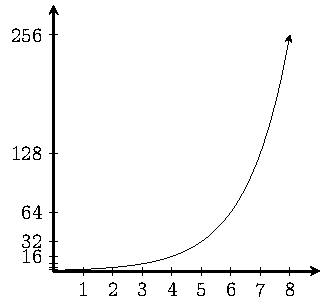
\includegraphics{basicderivativesandintegrals/exponentials}
    \caption{Exponential function $2^x$ plotted from $0$ to $8$}
    \label{fig:exponentialgraph}
\end{figure}
Notice that on the right most column of \cref{tab:exponentialbase2}, the difference between $V(t)$ and $V(t - 1)$ is exactly $V(t - 1)$: the function changes as much as its past-self. So does that mean that $\odv*{(2^x)}{x} = 2^x$?

Well sadly not, but close. See, \cref{tab:exponentialbase2} only shows a \emph{discrete} step. You can write it out as
\begin{equation}
    \frac{2^{x + 1} - 2^x}{1} = 2^x\left(\frac{2 - 1}{1}\right) = 2^x,
\end{equation}
that is why $V(t) - V(t - 1) = V(t - 1)$. But we still need the method of increments to calculate the derivative of $2^x$:
\begin{align*}
    \odv*{(2^x)}{x} &= \lim_{h \appr 0}\frac{2^{x + h} - 2^x}{\odif{x}} \\
    &= 2^x\lim_{h \appr 0}\left(\frac{2^h - 1}{h}\right).
\end{align*}
Now you could try plugging in a really small value of $h$, say $0.000001$. The term $\frac{2^h - 1}{h}$ will approach $0.69314\dots$. If you try other bases of exponents, say $3$, you might see a pattern emerging.
\begin{equation}
    \odv*{(3^x)}{x} = 3^x\lim_{h \appr 0}\frac{3^h - 1}{h}.
\end{equation}
\emph{The rate of change of an exponential function is always itself times a proportionality constant}. For $3^x$, it's about $1.09851\dots$. If we could find a number $n$ where $\frac{n^h - 1}{h} = 0$, we'd have a very pretty function which it is its own derivative. So let's find that!
 
\subsection{A function that is its own derivative}
\label{sec:function_equals_own_derivative}

Let's set a goal: find the function that is its own derivative. I shall introduce a substantial concept in calculus: the expansion of functions. Every function has a polynomial expansion\footnote{Although the convergence of the series derived is quite questionable; thankfully, the power series of $n^x$ converges everywhere.} called the \index{power series!introduction}\textbf{power series}. For every $f(x)$,
\begin{equation}
    f(x) = a_0 + a_1x^1 + a_2x^2 + a_3x^3 +\dots. \label{eq:naivetaylorseries}
\end{equation}
E.g., $\sin(x)$ can be written as
\begin{equation}
    \sin(x) = x - \frac{1}{3!}x^3 + \frac{1}{5!}x^5 - \frac{1}{7!}x^7 + \dots. \label{eq:taylorseriessine}
\end{equation}
we will derive this expression later in \cref{sec:sine_cosine_power_series}. For now, we can just use \cref{eq:naivetaylorseries} to find the expression for the function that is its own derivative.

We've seen that the exponential is a possible candidate for a function that is its own derivative. Now, assume that for some real number $n$,
\begin{equation}
    \odv*{(n^x)}{x} = n^x.
\end{equation}
Then, we use the polynomial expansion and the power rule,
\begin{align*}
    \odv*{(a_0 + a_1x^1 + a_2x^2 + a_3x^3 + \dots)}{x} &= a_1 + 2a_2x^1 + 3a_3x^2 + 4a_4x^3 + \dots \\
    &= n^x
\end{align*}
If the function is its own derivative, the polynomial expansion of the function and its derivative must be the same.
\begin{gather}
    n^x = a_0 + a_1x^1 + a_2x^2 + a_3x^3 + \dots, \label{eq:naivetaylorseries1}\\
    n^x = a_1 + 2a_2x^1 + 3a_3x^2 + 4a_4x^3 + \dots. \label{eq:naivetaylorseries2}
\end{gather}
Since both are polynomials, we can match the coefficient here:
\begin{equation}
    \begin{array}{c}
    a_0 = a_1 \\ a_1 = 2a_2 \\ a_2 = 3a_3 \\ a_3 = 4a_4 \\ \vdots
    \end{array}\label{eq:naivetaylorserieserelations}
\end{equation}
$a_0$ and $a_1$ is relatively easy to find. As we've seen, $n$ must be between $2$ and $3$. By the properties of exponentials, $x = 0 \implies n^x = 1$. We can then plug $x = 0$ and set $n^x = 1$ into \cref{eq:naivetaylorseries2}:
\begin{align*}
    1 &= a_0 + a_1(0)^1 + a_2(0)^2 + a_3(0)^3 + \dots \\
    a_0 &= 1.
\end{align*}
Since $a_0 = a_1$, $a_1$ must also be $1$. We can then go back to \cref{eq:naivetaylorserieserelations} and get
\begin{equation*}
    n^x = 1 + 1 + \frac{1}{2!}x + \frac{1}{3!}x^3 + \frac{1}{4!}x^4 + \dots
\end{equation*}
The pattern here is clearly $a_n = n!$. If we want to find $n$, we just let $x = 1$.
\begin{equation*}
    n = 1 + 1 + \frac{1}{2!} + \frac{1}{3!} + \frac{1}{4!} + \dots,
\end{equation*}
and there we have an expression for $n$ which is an irrational number. If you work this out, it's around $2.71828\dots$. Because $(2.71828\dots)^x$ is its own derivative, it's very useful in mathematics and appears everywhere, even at the seams of mathematics that doesn't even seems related to growths: the patterns of prime number, this constant $2.71828\dotso$ has a name and symbol: the Euler's number\footnote{Not to be confused with the ``Euler's constant'' which is another constant written $\gamma$, and is around $0.57721\dots$}, written as $\e$ where
\begin{equation}
    \e = \sum_{i = 0}^{\infty}\frac{1}{i!}
\end{equation}

\subsection{\protect Another interpretation of $\e$: infinite bank interests}

There are two types of bank interests: simple and compound. Simple interests is the thing that you don't really want: the interest is always the same and doesn't grow with your account. You can calculate it by using
\begin{equation}
    n(t) = n_0 + tr
\end{equation}
where $n(t)$ is the total money at time $t$, $n_0$ the initial money in your bank account, and $r$, the interest rate.

Compound interest in the other hand calculates your interest based on how much money you have at that moment:
\begin{equation}
    n(t + 1) = n(t)r + n(t).
\end{equation}
We can find the expression for $n(t)$ in a similar fashion to what we've done in \cref{eq:exponentialsrecurrencerelations}. You'll get
\begin{equation}
    n(t) = (1 + r)^tn_0 \label{eq:compoundinterestformula}
\end{equation}
which is an exponential function.

Let's say you deposit $100\$$ into a bank and the bank is offering you two options on \index{compound interest}\textbf{compound interests} rate. \begin{enumerate*}[label = \arabic*)]\item Take $100\%$ interest in $1$ year, \item Take $\flatfrac{100}{2}\%$ twice a year, or \item Take $\flatfrac{100}{356}\%$ daily.\end{enumerate*} If you take option one, you'd end up with $200\$$. Option two takes you to $225\$$, and option three takes you to around $271.447\dots\$$. You might see a theme here. If you get $\flatfrac{100}{n}\%$ interest, $n$ times a year, the result keeps getting higher. Is there an upper limit to this?

If we write it in terms of limits as $n \appr \infty$ and use \cref{eq:compoundinterestformula}, the compound interests formula,
\begin{equation*}
    x = \lim_{n \appr \infty}\left(1 + \frac{1}{n}\right)^nn_0.
\end{equation*}
Where $x$ is the total money after a year. We're interested in the upper limit, so we'll just let $n_0$ for now. The expression will become
\begin{equation}
    x = \lim_{n \appr \infty}\left(1 + \frac{1}{n}\right)^n \label{eq:infinitecompoundinterest}
\end{equation}
Technically, we could go in and substitute a very high $n$, such as $1000000$. But I believe you could already see that it would be a nightmare to calculate: exponentiation is not at all an easy task. However, notice that from option three earlier, the total money is $271.447\dots\$$ which is suspiciously similar to $\e$ at $2.71828\dots$. If \cref{eq:infinitecompoundinterest} equals \cref{eq:naivetaylorserieserelations}, we'd find the upper limit for this problem and solve the mystery.

We can use the binomial theorem on \cref{eq:infinitecompoundinterest} and get
\begin{align*}
    &\lim_{n \appr \infty}\sum_{k = 0}^{n}{n \choose k}1^{n - k}\frac{1}{n^k} \\
    &= \lim_{n \appr \infty}{n \choose 0}\frac{1}{n^0} + {n \choose 1}\frac{1}{n^1} + {n \choose 2}\frac{1}{n^2} + {n \choose 3}\frac{1}{n^3} + \dots.
\end{align*}
Then, we use the definition of $n$ choose $k$,
\begin{align*}
    &= 1 + \lim_{n \appr \infty}\frac{n!}{1!(n - 1)!}\frac{1}{n^1} + \frac{n!}{2!(n - 2)!}\frac{1}{n^2} + \frac{n!}{3!(n - 3)!}\frac{1}{n^3} + \dots.
\end{align*}
Now, we can cancel the $n!$ on the numerator to the denominator and isolate the factorials.
\begin{align*}
    &= 1 + \lim_{n \appr \infty}\frac{n(n - 1)!}{(n - 1)!}\frac{1}{1!n^1} + \frac{n(n - 1)(n - 2)!}{(n - 2)!}\frac{1}{2!n^2} + \dots \\
    &= 1 + \frac{1}{1!} + \lim_{n \appr \infty} \frac{n(n - 1)}{2!n^2} + \frac{n(n - 1)(n - 2)}{3!n^3} + \frac{n(n - 1)(n - 2)(n - 3)}{4!n^4} + \dots
\end{align*}
Notice, as $n \appr \infty$, the ratio between $n + R$ and $n$ where $R$ is any real numbers would be literally negligible. For every terms in our series, both the numerator and the denominator has the same polynomic degrees. Therefore, all the $n$'s in the series cancel out and we get
\begin{equation}
    x = 1 + \frac{1}{1!} + \frac{1}{2!} + \frac{1}{3!} + \dots
\end{equation}
which is literally \cref{eq:naivetaylorserieserelations}; thus,
\begin{equation}
	\e = \lim_{n \appr \infty}\ab(1 + \frac{1}{n})^n. \label{eq:e-def-infinite-interests}
\end{equation}

In conclusion, the upper limit that the bank can give you is $\e$, which should make sense geometrically. Because we're gradually turning a discrete interest into a continuous one, $\e$ should appear in the limit of the continuous bank interests.

The limit definition of $\e$ allows us to express $\e^x$ in terms of limits.
\begin{align}
	\e^x &= \ab(\lim_{n \appr \infty}\ab(1 + \frac{1}{n})^n) \\
		 &= \lim_{n \appr \infty}\ab(1 + \frac{1}{n})^{nx}
\end{align}
If $n = \flatfrac{u}{x}$, then
\begin{align}
	\e^x &= \lim_{\frac{u}{x} \appr \infty}\ab(1 + \frac{u}{h})^{h}
\end{align}
For $\frac{u}{x} \appr \infty$ to be true for all finite $x$, $u$ must approach $\infty$; therefore,
\begin{align}
	\e^x &= \lim_{u \appr \infty}\ab(1 + \frac{u}{h})^h
\end{align}

\subsection{The antiderivative of exponential functions}

It should be trivial that if $\e^x$ is the derivative of itself, so is its antiderivative
\begin{equation}
    \int \e^x \odif{x} = \e^x + C.
\end{equation}
For other bases, we could use the fundamental theorem of calculus (\cref{theorem:fundamentalthmofcalc1}) to find its antiderivative. I.e., if
\begin{equation*}
    \odv{(n^x)}{x} = n^x\lim_{h \appr 0}\frac{n^h - 1}{h},
\end{equation*}
then
\begin{align*}
    \odv*{(n^x)}{x} &= n^x\lim_{h \appr 0}\frac{n^h - 1}{h} \\
    n^x &= \lim_{h \appr 0}\frac{n^h - 1}{h}\int n^x\odif{x} \\
    \int n^x\odif{x} &= n^x\lim_{h \appr 0}\left(\frac{n^h - 1}{h}\right)^{-1} + C.
\end{align*}
The term in the limit sign still appears here. If we want to uncover the origin of this term, we must discuss the logarithms.

\section{Logarithms}

Logarithms are inverses of exponential, like how roots are inverses of monomials. To illustrate what I mean,
\begin{equation*}
	\textrm{For monomials, } \sqrt[a]{x^a} = x, \textrm{ but with logarithms, } \log_{a}(a^x) = x.
\end{equation*}
They have the following properties:
\begin{gather}
    \log_a(x) + \log_a(y) = \log_a(xy), \\
    \log_a(x) - \log_a(y) = \log_a\left(\frac{x}{y}\right), \\
    \log_a(x) = \frac{\log_b(x)}{\log_b(a)}.
\end{gather}
Since $\e^x$ is shown to be a very important function in modelling continuous growth, and is its own derivative, we give its inverse function its own name: the \index{logarithms!natural logarithms}\textbf{natural logarithm}, written as $\ln(x)$.

What's the derivative of $\ln(x)$? By the method of increments,
\begin{align}
	\odv*{\ln(x)}{x} &= \lim_{h \appr 0}\frac{\ln(x + h) - \ln(x)}{h} \\
					&= \lim_{h \appr 0}\frac{\ln(\frac{x + h}{x})}{h} \\
					&= \lim_{h \appr 0}\frac{\ln(1 + \frac{h}{x})}{h} \\
					&= \lim_{h \appr 0}\ln\ab(\ab(1 + \frac{h}{x})^{\frac{1}{h}}).
\end{align}
This form is very similar to the limit definition of the exponential function $\e^x$, but with some terms swapped around. So let's try to fit this limit to the form of $\e^x$. I shall let $h = \frac{1}{n}$. If $h \appr 0$, then $n \appr \infty$. Therefore,
\begin{align}
	\odv*{\ln(x)}{x} &= \lim_{n \appr \infty}\ln\ab(\ab(1 + \frac{1}{nx})^{n}) \\
					 &= \lim_{n \appr \infty}\ln\ab(\ab(1 + \frac{\flatfrac{1}{x}}{n})^n). \label{eq:ln-diff-derivation}
\end{align}
Recall that
\begin{equation}
	\e^x = \lim_{n \appr \infty}\ab(1 + \frac{x}{n})^n.
\end{equation}
Thus,
\begin{equation}
	\lim_{n \appr \infty}\ab(1 + \frac{\flatfrac{1}{x}}{n})^n = \e^{\frac{1}{x}}.
\end{equation}
which fits the form of \cref{eq:ln-diff-derivation}. Therefore,
\begin{align}
	\odv*{\ln(x)}{x} &= \lim_{n \appr \infty}\ln(\e^{\frac{1}{x}}) \\
					 &= \lim_{n \appr \infty}\frac{1}{x} = \frac{1}{x}:
\end{align}
the derivative of the natural logarithm of $x$ is the reciprocal of $x$.

This result can also be interpretted geometrically. If the exponential grows very quickly when $x$ increases, its inverse must grow slow. The slow growing rate is directly captured by the function $\frac{1}{x}$.

Here is the perfect time that I'll give you a glimpse into calculus with many variables: multivariable calculus. I shall present another way to derive the derivative of $\ln(x)$: \textbf{implicit differentiation}.\index{implicit differentiation}

Functions in the form $f(x) = y$ are called \textbf{explicit functions}: the relations between the two variables are written explicitly. Functions that can't be written as $f(x) = y$ are called \textbf{implicit functions}, e.g., $x^2 + y^2 = r^2$. \textbf{Implicit differentiation} concerns the differentiation of implicit functions. In this case, it actually makes our life easier if we turn $\ln(x)$ into an implicit function.

If I let $\ln(x) = y$, I can raise both sides to the power of $\e$ and get
\begin{equation}
    \e^{\ln(x)} = \e^y.
\end{equation}
Because logarithms are inverses of exponential,
\begin{equation}
    x = \e^y.
\end{equation}
By the rule of equality, (\cref{sec:trivial_rules}), we can take the derivative of both sides w.r.t. $y$ instead of $x$:
\begin{align*}
    \odv{x}{y} &= \odv{\e^y}{y} \\
    \odv{x}{y} &= \e^y.
\end{align*}
But we're looking for the derivative of $y$ (which is just $\ln(x)$) w.r.t. $x$, not the derivative of $x$ w.r.t. $y$. Here's where Leibniz's notation comes into clutch: we can swap the numerator with the denominator for both sides then, substitute back $y = \ln(x)$:
\begin{align*}
    \odv{\ln(x)}{x} &= \frac{1}{\e^{\ln(x)}} \\
    \therefore~\odv{\ln(x)}{x} &= \frac{1}{x},
\end{align*}
and there: the derivative of the natural logarithm is the reciprocal.

With the power of natural logarithms, we can actually go back at the derivative of $n^x$ and finally uncover the mystery behind the proportionality term that's lingering around. Start with the manipulation of $n^x$.
\begin{equation}
    n^x = \left(\e^{\ln(n)}\right)^x = \e^{x\ln(x)}.
\end{equation}
With the chain rule (\cref{sec:trivial_rules}), let $u = x\ln(n)$:
\begin{align*}
    \odv*{(n^x)}{x} &= \odv{\e^{x\ln(n)}}{x} \\
    &= \odv{\e^u}{x} \times \odv{u}{u} \\
    &= \odv{\e^u}{u} \times \odv{u}{x} \\
    &= \e^{x\ln(n)} \times \odv{x\ln(n)}{x} \\
    &= n^x\ln(n).
\end{align*}
And here it is: the mystery proportionality constant. It's just a consequence of the natural logarithm. Thus, one way to define the natural log would be
\begin{equation}
    \ln(n) = \lim_{h \appr 0}\frac{n^h - 1}{h}.
\end{equation}
The antiderivative of other bases exponents are then given by
\begin{equation}
    \int n^x = \frac{1}{\ln(n)}n^x + C.
\end{equation}

\subsection{The product rule and the quotient rule}
\index{derivatives!product rule}

Sometimes, we have to multiply the two functions together before taking the derivatives. There are two ways to do this. To keep the spirit of visualization, I shall first introduce the geometrical way, then the analytical way.

\begin{figure}[h]
    \centering
    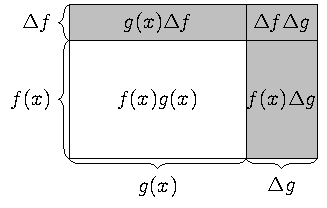
\includegraphics{basicderivativesandintegrals/derivativesproductrule}
    \caption{The geometrical interpretation of the product rule.}
    \label{fig:derivativesproductrule}
\end{figure}
The derivative of $f(x)g(x)$ w.r.t. $x$ can be thought of a rectangle with side length that's governed by $f(x)$ and $g(x)$. As shown in \cref{fig:derivativesproductrule}, the area increase on side $f(x)$ is $g(x)\Dd{f}$ and on $g(x)$, $f(x)\Dd{g}$. The $\Dd{f}\Dd{g}$ part is basically negligible. Therefore,
\begin{align*}
    \odv*{\ab(f(x)g(x))}{x} &= \lim_{h \appr 0}\frac{g(x)\Dd{f} + f(x)\Dd{g}}{h} \\
    &= \lim_{h \appr 0}\frac{f(x)(g(x + h) - g(x)) + g(x)(f(x + h) - f(x))}{h} \\
    &= f(x)\lim_{h \appr 0}\frac{g(x + h) - g(x)}{h} + g(x)\lim_{h \appr 0}\frac{f(x + h) - f(x)}{h} \\
    &= f(x)\odv{g(x)}{x} + g(x)\odv{f(x)}{x}.
\end{align*}
Which is what we call the product rule. Notice the alternation between $f$ and $g$ in the two terms. The derivative of $f(x)$ is multiplied by $g(x)$, and the derivative of $g(x)$ is multiplied by $f(x)$. This is a direct consequence of the diagram: the change in $f(x)$ is multiplied by $g(x)$ to give the area and also the other way around. You could check this with the method of increments, and it would still be true. I encourage you to do it.

\index{derivatives!quotient rule}To take derivatives of quotients of functions, just plug in $\flatfrac{1}{g(x)}$ instead of $g(x)$. The final form should be
\begin{equation}
    \odv*{\ab(\frac{f(x)}{g(x)})}{x} = \frac{\displaystyle f(x)\odv{g(x)}{x} - g(x)\odv{f(x)}{x}}{f(x)^2}.
\end{equation}
But how's about the product of multiple functions? We can't really geometrically interpret those anymore. So we have to turn ourselves to the analytical method.

Let's think of this through. We don't know the derivative of products, but we know the derivative of \emph{sums}: the linearity property. So if we can turn products into sum, this problem would be so easy! Gladly, the logarithms can do exactly that. To make our life easier, we shall use the natural logarithm. Because I want to save space, let's write $a(x)b(x)c(x)$ as just $abc$. Do know that these functions are all dependent on $x$. Start off with a manipulation of products.
\begin{align*}
    \odv{(abc\dots)}{x} &= \odv*{(\e^{\ln(abc\dots)})}{x} \\
    &= \odv*{(\e^{\ln(a) + \ln(b) + \ln(c) + \dots})}{x}.
\end{align*}
Now, let $\ln(a) + \ln(b) + \ln(c) + \dots = u$ and use the chain rule,
\begin{align*}
    &= \odv*{(\e^u)}{x} \cdot \odv{u}{u} \\
    &= \odv*{(\e^u)}{x} \cdot \odv*{\ab(\ln(a) + \ln(b) + \ln(c) + \dots)}{x} \\
    &= \e^u \left(\odv{\ln(a)}{x} + \odv{\ln(b)}{x} + \odv{\ln(c)}{x} + \dots\right).
\end{align*}
Then use the chain rule again on the terms in the parenthesis
\begin{align*}
    &= \e^u \left(\odv{\ln(a)}{x}\odv{a}{a} + \odv{\ln(b)}{x}\odv{b}{b} + \odv{\ln(c)}{x}\odv{c}{c} + \dots\right) \\
    &= (abc\dots)\left(\odv{\ln(a)}{a}\odv{a}{x} + \odv{\ln(b)}{b}\odv{b}{x} + \odv{\ln(c)}{c}\odv{c}{x} + \dots\right) \\
    &= (abc\dots)\left(\frac{1}{a}\odv{a}{x} + \frac{1}{b}\odv{b}{x} + \frac{1}{c}\odv{c}{x} + \dots\right).
\end{align*}
And there we have it: the generalized product rule.

\subsection{Alternative derivations for the power rule}

The power rule can also be derived using the same technique we just used. However, we use a different property of logarithm: $\ln(x^n) = n\ln(x)$.
\begin{equation*}
    \odv*{x^n}{x} = \odv*{\e^{n\ln(x)}}{x}.
\end{equation*}
Let $u = n\ln(x)$ then use the chain rule
\begin{align*}
    &= \odv{\e^u}{x} \cdot \odv{u}{u} \\
    &= \odv{\e^u}{u} \cdot \odv{u}{x} \\
    &= \e^u \cdot \odv*{\ab(n\ln(x))}{x} \\
    &= x^n \cdot n\frac{1}{x} = nx^{n - 1}.
\end{align*}

\section{Implicit differentiation}

Implicit differentiation also shows up in problems where two rate of changes are related to each other: the \textbf{related rates} problem. Consider a sliding ladder that's $5\unit{\meter}$ long (\cref{fig:slidingladder}). At a certain time $t$, what's the sliding rate along the $x$-axis w.r.t. the $y$-axis?\index{related rates}

\begin{figure}
    \centering
    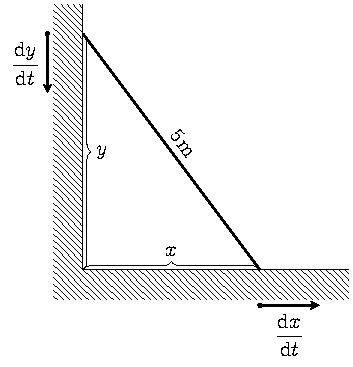
\includegraphics{basicderivativesandintegrals/slidingladder}
    \caption{A ladder length $5\unit{\meter}$ sliding down a corner.}
    \label{fig:slidingladder}
\end{figure}

The problem is asking for $\odv{x}{y}$. Here, the rate of sliding along the $y$-axis $\odv{y}{t}$ and along the $x$-axis $\odv{x}{t}$ is related because the ladder length is fixed. If $y$ decreases, $x$ must increase. The Pythagorean theorem says
\begin{equation}
    x^2 + y^2 = 5^2.
\end{equation}
We can take the derivative w.r.t. $t$ on both side then use the chain rule
\begin{align*}
    \odv{x^2}{t} + \odv{y^2}{t} &= \odv{(5^2)}{t} \\
    \odv{x^2}{x}\odv{x}{t} + \odv{y^2}{y}\odv{y}{t} &= 0 \\
    2x\odv{x}{t} + 2y\odv{y}{t} &= 0.
\end{align*}
We can take advantage of the Leibniz's notation and multiply by $\odif{t}$ on both sides giving
\begin{equation*}
    2x\odif{x} + 2y\odif{y} = 0.
\end{equation*}
To find $\odv{x}{y}$, we just have to isolate the variables,
\begin{align*}
    \odv{x}{y} = -\frac{y}{x}.
\end{align*}
And this should actually make sense. Because if $y$ is increasing by a bit, $x$ must decrease by some amount, and that amount is $-\flatfrac{y}{x}$: the higher the $y$, the larger the rates of sliding.

\section{Technique of integraton: substitution}

Before we finish this chapter off, I'd want to take a look at a very useful technique for dealing with complicated integrals: substitution.

Substitution is a technique to simplify algebraic expressions. I believe you've already seen a multitude of them. Basically, we substitute some expression of $x$ with $u$, then use everything in our power to change every $x$ to $u$, including the differential element: from $\odif{x}$ to $\odif{u}$.

$u$-substitution works when the integrals are of the form
\begin{equation}
	\int f\ab(g(x))\odv{g(x)}{x}\odif{x}.
\end{equation}
In this notation, it's easy to see that the $\odif{x}$ will cancel, leaving us with
\begin{equation}
	\int f\ab(g(x))\odif{g(x)}.
\end{equation}
If $g(x) = u$, then our integral simplifies to
\begin{equation}
	\int f(u)\odif{u}.
\end{equation}

Let's apply this knowledge to solve some integrals. Starting with the simplest: polynomic integrands.
\begin{exmp}{$\int x(x^2 + 1)^{10}\odif{x}$}{u-substitution-1}
	If $f(x) = x^{10}$, and $u = x^2 + 1$, then
	\begin{equation}
		\int x(x^2 + 1)^{10}\odif{x} = \int u^{10}x\odif{x}.
	\end{equation}
	Because $x = \frac{1}{2}\odv{(x^2 + 1)}{x}$,
	\begin{equation}
		\int u^{10}x\odif{x} = \int u^{10}\frac{1}{2}\odv{(x^2 + 1)}{x}\odif{x} = \frac{1}{2}\int u^{10}\odif{(x^2 + 1)}
	\end{equation}
	Since $u = x^2 + 1$, our integral simplifies to
	\begin{equation}
		\frac{1}{2}\int u^{10}\odif{u}.
	\end{equation}
	Using the reversed power rule (\cref{eq:power_rule}), we get
	\begin{equation}
		\frac{1}{2}\frac{u^{11}}{11} = \frac{u^{11}}{22} = \frac{(x^2 + 1)^{11}}{22} + C.
	\end{equation}
\end{exmp}

\begin{exmp}{$\int x^2\e^{4x^3 + 4}\odif{x}$}{u-substitution-3}
	The integrand is a composite function: $f(u) = \e^u$ and $u = 4x^3 + 4$. In which, $\odv{u}{x} = 12x^2$; therefore,
	\begin{align}
		\int x^2\e^{4x^3 + 4}\odif{x} &= \frac{1}{12}\int\e^u 12x^2 \odif{x} \\
										&= \frac{1}{8}\int\e^u\odv{u}{x}\odif{x} \\
										&= \frac{1}{8}\int\e^u\odif{u} = \frac{1}{8}\e^u \\
										&= \frac{1}{12}\e^{4x^3 + 4} + C.
	\end{align}
\end{exmp}

Notice any patterns? If the integral has a polynomial $u$ with degree $n$ nested inside another function, there must be a term outside with the degree $n - 1$ to substitute with. In \cref{exmp:u-substitution-1}, $u = x^2 + 1$ and there's an $x$ multiplied outside waiting to be substituted. In \cref{exmp:u-substitution-3}, $u = 4x^3 + 4$, and there's an $x^2$ outside. This pattern is a consequence of the power rule, and is pretty common. So, here are some practice problems with answers and hints on the right.\footnote{Practice problems taken from \cite{foster-no-date}.} Try not to look at it much.

\begin{enumerate}
	\item $\int 3x^2\sqrt{x^3 + 5}\odif{x}$ \hfill $\frac{2}{3}(x^3 + 5)^{\frac{3}{2}} + C$, $u = x^3 + 5$
	\item $\int \sqrt{4 + 3x}\odif{x}$ \hfill $\frac{2}{9}(3x + 4)^{\frac{3}{2}} + C$, $u = 4 + 3x$
	\item $\int \frac{24x}{(4x^2 + 4)^2}\odif{x}$ \hfill $\frac{3}{4x^2 + 4} + C$, $u = 4x^2 + 4$
\end{enumerate}

Now let's move on from polynomials to other functions that are nested inside another function. For the substitution to work, there must be the function's derivative multiplied, waiting to be substituted. A classic example is:
\begin{exmp}{$\int \frac{\ln(x)}{x}\odif{x}$}{u-substitution-3}
	This integral is not quite a composite function, but rather just a product between a function and its derivative. If $u = \ln(x)$, then $\odv{u}{x} = \frac{1}{x}$; therefore,
	\begin{align}
		\int \frac{\ln(x)}{x}\odif{x} &= \int u\odv{u}{x}\odif{x} \\
									  &= \int u\odif{u} \\
									  &= \frac{u^2}{2} = \frac{\ln(x)^2}{2} + C.
	\end{align}
\end{exmp}

\begin{exmp}{$\int x\e^{x^2}(\e^{x^2} + 3)\odif{x}$}{u-substitution-4}
	Let $\e^{x^2} + 3 = u$, then
	\begin{align}
		\odv{u}{x} &= \odv{\e^{x^2} + 3}{x} \\
				   &= \odv{\e^{x^2}}{x} \\
				   \intertext{Let $x^2 = v$, then by the chain rule,}
				   &= \odv{\e^v}{x} \cdot \odv{v}{v} \\
				   &= \odv{\e^v}{v} \cdot \odv{x^2}{x} \\
				   &= 2x\e^v = 2x\e^{x^2}.
	\end{align}
	Thus,
	\begin{align}
		\int x\e^{x^2}(\e^{x^2} + 3)\odif{x} &= \frac{1}{2}\int u\ab(2x\e^{x^2})\odif{x} \\
											 &= \frac{1}{2}\int u\odv{u}{x}\odif{x} = \frac{1}{2}\int u\odif{u} \\
											 &= \frac{1}{2}\frac{u^2}{2} = \frac{(\e^{x^2} + 3)^2}{4} + C.
	\end{align}
\end{exmp}

Sometimes, they need some \emph{creative} algebraic manipulations, and sometimes even multiple substitution. E.g.,\footnote{Taken from MIT Integration Bee 2019, $I_9$ \cite{alkousa-2023}}
\begin{exmp}{$\frac{1}{x(x^5 + 1)}\odif{x}$}{u-substitution-5}
	If we want to use power rule substitution, there's only $x^5$ but no $x^4$ to substitute with. So, we need to get a bit creative.

	First, factor the $x^5$ out of the inner parenthesis and get
	\begin{equation}
		\int\frac{1}{x^6\ab(1 + \frac{1}{x^5})}\odif{x}.
	\end{equation}
	Now, we can let $u = 1 + \frac{1}{x^5}$. By the power rule, $\odv{u}{x} = -\frac{5}{x^6}$. Our integral then becomes
	\begin{align}
		-5\int\frac{1}{u}\ab(-\frac{5}{x^6})\odif{x} &= -\frac{1}{5}\int\frac{1}{u}\odv{u}{x}\odif{x} \\
													 &= -\frac{1}{5}\int\frac{1}{u}\odif{u} = -5\ln(x) \\
													 &= -\frac{1}{5}\ln\ab(1 + \frac{1}{x^5}) + C
	\end{align}
\end{exmp}

In certain problems, there aren't any outside terms to substitute with, so you have to create them. E.g.,
\begin{exmp}{$\int\ab(1 + \sqrt{x})^4\odif{x}$}{}
	We want to get rid of the term inside the parenthesis. So, let $u = 1 + \sqrt{x}$, and by the power rule, $\odv{u}{x} = \frac{1}{2\sqrt{x}}$. However, there is no $\frac{1}{\sqrt{x}}$ outside to substitute with. Let's be adventurous and substitute $u$ in anyways and see what happens.
	\begin{align}
		\int(1 + \sqrt{x})^4\odif{x} &= \int u^4\odif{x}
		\intertext{If $\odv{u}{x} = \frac{1}{2\sqrt{x}}$, then $\odif{x} = 2\sqrt{x}\odif{u}$,}
									 &= \int u^4\ab(2\sqrt{x})\odif{u}.
	\end{align}
	We're almost there, now we just have to replace the leftover $x$ with $u$. Since $u = 1 + \sqrt{x}$, $\sqrt{x} = u - 1$; thus,
	\begin{align}
		\int u^4\ab(2\sqrt{x})\odif{u} &= 2\int u^4(u - 1)\odif{u} \\
									   &= 2\int u^5 - u^4\odif{u} = 2\ab(\frac{u^6}{6} - \frac{u^5}{5}) \\
									   &= 2\ab(\frac{(1 + \sqrt{x})^6}{6} - \frac{(1 + \sqrt{x})^5}{5}).
	\end{align}
\end{exmp}

These problems definitely take a while to get used to. So I highly encourage you to practice integrating using a problem set (\cite{alkousa-2023}, \cite{foster-no-date}). The unfortunate thing is that most problem sets include trigonometry. So, you'd have to pick the one without them to practice with. Or, you can just wait until we discuss about trigonometry and then practice from there.

\section{Integral of the reciprocal}
\label{sec:integralofthereciprocal}

\index{integrals!integrals of the reciprocal}
% \begin{wrapfigure}{r}{0.45\textwidth}
%     \centering
%     \begin{tabular}{c | c}
%         Function & Antiderivative \\
%         \hline
%         $x^{-3}$ & $-\flatfrac{x^{-2}}{2}$ \\
%         $x^{-2}$ & $x^{-1}$ \\
%         $x^{-1}$ or $\flatfrac{1}{x}$ & $\ln(x)$ \\
%         $x^{0}$ or $1$ & $x$ \\
%         $x^1$ & $\flatfrac{x^2}{2}$ \\
%     \end{tabular}
%     \caption{Tables of reversed power rule from $x^{-3}$ to $x^1$}
% \end{wrapfigure}
By the fundamental theorem of calculus (\cref{theorem:fundamentalthmofcalc1}), the antiderivative of $\frac{1}{x}$ is $\ln(x)$. You might believe this, and it's not wrong. But I find it very disturbing and unresolved. It's like taking the result and pointing it back to the origin. It doesn't really make sense. So from this dissatisfaction, I spent a night coming up with a way to derive this using just the reversed power rule. Enjoy the transformation!
\begin{align}
	\int \frac{1}{x}\odif{x} &= \int\lim_{h \appr 0}\left(\frac{1}{2}x^{-1 + h} + \frac{1}{2}x^{-1 - h}\right)\odif{x} \nonumber\\
							 &= \lim_{h \appr 0}\int\left(\frac{1}{2}x^{-1 + h} + \frac{1}{2}x^{-1 - h}\right)\odif{x} \nonumber\\
							 &= \lim_{h \appr 0}\int\left(\frac{1}{2}\frac{x^{-1 + h + 1}}{(-1 + h + 1)} + \frac{1}{2}\frac{x^{-1 - h + 1}}{(-1 - h + 1)}\right)\odif{x} \nonumber\\
    &= \lim_{h \appr 0}\left(\frac{1}{2}\frac{x^h}{h} - \frac{1}{2}\frac{x^{-h}}{-h}\right) = \lim_{h \appr 0}\left(\frac{1}{2}\frac{x^h}{h}\frac{x^h}{h} - \frac{1}{2}\frac{1}{hx^h}\right) \nonumber\\
    &= \lim_{h \appr 0}\left(\frac{x^{2h} - 1}{2hx^h}\right) = \lim_{h \appr 0}\left(\frac{\e^{2h\ln(x)} - 1}{2h\ln(x)}\cdot\frac{\ln(x)}{x^h}\right) \nonumber\\
    &= \lim_{h \appr 0}\left(\frac{\e^{2h\ln(x)}}{2h\ln(x)}\right) \cdot \lim_{h \appr 0}\left(\frac{\ln(x)}{x^h}\right) \nonumber\\
    &= \lim_{h \appr 0}\left(\frac{\e^{2h\ln(x)}}{2h\ln(x)}\right) \cdot \ln(x). \label{eq:logarithmsprove1}
\end{align}
Then, we evaluate the limit at the front by letting $u = 2h\ln(x)$. When $h \appr 0$, $u \appr 0$ as well. Then, use the definition of $\e$ from \cref{eq:infinitecompoundinterest}.
\begin{align*}
    \lim_{h \appr 0}\left(\frac{\e^{2h\ln(x)}}{2h\ln(x)}\right) &= \lim_{u \appr 0}\left(\frac{\e^u - 1}{u}\right) \\
    &= \lim_{u \appr 0}\left(\frac{\left(\lim_{n \appr \infty}\left(1 + \frac{1}{n}\right)^n\right)^u}{u}\right).
\end{align*}
Change the limits from $n \appr \infty$ into $n \appr 0$. Notice, $\lim_{n \appr 0}\left(1 + \frac{1}{n}\right)^n = \lim_{n \appr 0}\left(1 + n\right)^{\flatfrac{1}{n}}$. If $n \appr 0$ and $u \appr 0$, that means $n = u$. Substitute $n = u$ into the limit,
\begin{align*}
    &= \lim_{u \appr 0}\left(\frac{\left(\lim_{u \appr 0}(1 + u)^{\flatfrac{1}{u}}\right)^u - 1}{u}\right) \\
    &= \lim_{u \appr 0}\left(\frac{1 + u - 1}{u}\right) = 1.
\end{align*}
Then, substitute this limit back into \cref{eq:logarithmsprove1}, you'll see that
\begin{equation*}
    \int\frac{1}{x}\odif{x} = \lim_{h \appr 0}\left(\frac{\e^{2h\ln(x)}}{2h\ln(x)}\right) \cdot \ln(x) = \ln(x) + C,
\end{equation*}
completing the proof.

\section{Formula for Chapter \thechapter}

\everymath{\displaystyle}
\subsection{Formula for derivatives of functions}

\begin{enumerate}
    \item $f(x) = g(x) \implies \odv{f(x)}{x} = \odv{g(x)}{x}$ (Rules of Equality)
    \item For $c \in \mathbb{R}$, $\odv{(c)}{x} = 0$ (Derivative of a constant)
    \item $\odv{x}{y} = \odv{x}{u} \times \odv{u}{y}$ (Chain rule)
    \item $\odv*{\ab(af(x) + bg(x))}{x} = a\odv{f(x)}{x} + b\odv{g(x)}{x}$ (Linearity of differentiation)
    \item $\odv*{(ax^n)}{x} = anx^{n - 1}$ (Power rule)
    \item $\odv*{(n^x)}{x} = n^x\ln(n)$, $\odv{(\e^x)}{x} = \e^x$ (Derivative of exponentials)
    \item $\odv*{\ab(\ln(x))}{x} = \frac{1}{x}$ (Derivative of natural logarithms)
	\item $\odv*{\ab(f_1(x)f_2(x))}{x} = f_1(x)\odv{f_2}{x} + f_2(x)\odv{f_1}{x}$ (Product rule for two functions)
	\item $\odv*{(f_1f_2\dots f_n)}{x} = f_1f_2\dots f_n\ab(\frac{1}{f_1}\odv{f_1}{x} + \frac{1}{f_2}\odv{f_2}{x} + \dots + \frac{1}{f_n}\odv{f_n}{x})$ (Generalized product rule)
\end{enumerate}

\subsection{Formula for antiderivatives of functions}

\begin{enumerate}
    \item $f(x) = g(x) \implies \int f(x)\odif{x} = \int g(x)\odif{x}$ (Rules of Equality)
    \item $\int af(x) + bg(x) \odif{x} = a\int f(x)\odif{x} + b\int g(x)\odif{x}$ (Linearity of integration)
    \item $n \neq -1$, $\int ax^n\odif{x} = a\frac{x^{n + 1}}{n + 1} + C$ (Reversed power rule)
    \item $\int n^x\odif{x} = \frac{1}{\ln(n)}n^x + C$, $\int \e^x\odif{x} = \e^x + C$ (Antiderative of exponentials)
    \item $\int \frac{1}{x}\odif{x} = \ln(x) + C$ (Antiderivative of the reciprocal)
	\item $\int f(g(x))\odv{g}{x}\odif{x} = \int f(u)\odif{u}; u = g(x)$ ($u$-Substitution)
\end{enumerate}

\subsection{Definition for various functions and constants}

\begin{enumerate}
	\item $\e^x = \lim_{k \appr 0}\sum_{i \appr 0}^{k}\frac{1}{i!} = 1 + \frac{x^1}{1!} + \frac{x^2}{2!} + \frac{x^3}{3!} + \dots = \lim_{n \appr \infty}\ab(1 + \frac{x}{n})^n$
	\item $\e = \sum_{i = 0}^{\infty}\frac{1}{i!} = 1 + \frac{1}{1!} + \frac{1}{2!} + \frac{1}{3!} + \dots = \lim_{n \appr \infty}\left(1 + \frac{1}{n}\right)^n$
    \item $\ln(x) = \lim_{n \appr 0}\left(\frac{x^h - 1}{h}\right)$
\end{enumerate}

\everymath{\textstyle}
